\chapter{Strings, Gravitation, Kompaktifizierung und T-Dualität}

\lectureoverview{Ein Punktteilchen kann sich auf praktisch jeder glatten Geometrie konsistent bewegen, eine Quantensaite jedoch nicht. Ihre unendlich vielen Nullpunktschwingungen tasten den Zielraum auf immer kleineren Skalen ab, und die effektive Geometrie ändert sich, wenn diese Schwingungen wieder berücksichtigt werden. Die Forderung, dass dieser Prozess einen Fixpunkt besitzt, liefert \(R_{\mu\nu}=0\), die Vakuum-Einstein-Gleichung. Anschließend wenden wir uns von dieser Konsistenzbedingung der Kompaktifizierung zu. Ein Kreis ermöglicht sowohl Kaluza--Klein-Impulszustände als auch Saitenwicklungszustände. Durch ihren Austausch wird ein Kreis mit Radius \(R\) einem Kreis mit Radius \(\alpha'/R\) zugeordnet.}

\section{Konsistenz als Auswahlprinzip}

Zwei Fragen sind zu beantworten: Warum tritt Gravitation in der Stringtheorie auf, und warum lässt die Stringtheorie weit weniger Spielraum als die Mechanik von Punktteilchen? Im Grunde ist das eine einzige Frage. Eine Hintergrundgeometrie ist nur dann zulässig, wenn sich eine Saite auf ihr ausbreiten kann, ohne dass eine beliebige Abhängigkeit davon bestehen bleibt, wie fein wir die Saite auflösen.

Beginnen wir mit dem Kontrollproblem: einem Punktteilchen, das auf eine glatte gekrümmte Fläche beschränkt ist. Klassisch folgt es einer Geodäte, dem intrinsischen Gegenstück zu einer geraden Linie. Man kann die Bewegung durch viele kurze Abschnitte annähern, eine Differenzengleichung aufstellen und anschließend die Abschnittslänge gegen null gehen lassen. Das Ergebnis ist eine gewöhnliche Differentialgleichung mit einem wohldefinierten Kontinuumslimes.

Die Quantenmechanik verändert die Summe über die Pfade, nicht aber das Ergebnis. Statt einen einzigen klassischen Pfad auszuwählen, summieren wir Amplituden über Pfade auf der Fläche. Die Zeit lässt sich wiederum in kleine Schritte unterteilen; der Grenzfall wird gleichwertig durch eine Schr\"odinger-Gleichung auf dem gekrümmten Konfigurationsraum beschrieben. Bei einer glatten Fläche ergibt sich ein eindeutiger Propagator und ein eindeutiges Spektrum.

\begin{figure}[H]
  \centering
  \includegraphics[width=0.72\textwidth]{lecture_09_figure_01.png}
  \caption{Ein glatter Pfad auf der Fläche und ein gezackter Pfad aus der quantenmechanischen Zeit-Scheiben-Summe. Beide bleiben intrinsisch auf den Zielraum beschränkt.}
  \lectureframe{00:05:10}
  \label{fig:l09-particle-paths}
\end{figure}

\begin{classroomqa}
\audiencequestion{Müssen alle Pfade im Pfadintegral auf der Fläche bleiben? \lecturetimestamp{00:05:39}}
\lecturerresponse{Ja. Die Fläche ist der Konfigurationsraum des Teilchens, keine in einen größeren Raum eingebettete Fläche, durch die das Teilchen eine Abkürzung nehmen könnte. Jeder Zwischenpunkt liegt auf der Fläche, und alle Längen und Wirkungen werden mit ihrer intrinsischen Metrik berechnet.}
\end{classroomqa}

Die entsprechende Frage ist bei einer Saite schwieriger. Eine Saite wird nicht allein durch die Position ihres Schwerpunkts beschrieben. Sie besitzt eine unendliche Oszillatorturmstruktur. Eine höhere Auflösung bedeutet daher, weitere dynamische Freiheitsgrade zuzulassen. Die Theorie ist nur dann konsistent, wenn die Observablen bei Wiederherstellung dieses Turms gegen einen Grenzwert konvergieren.

\section{Das Punktteilchen auf einer Kugel}

Die Kugel ist die einfachste gekrümmte Testgeometrie. Sei ihr Radius \(R\); zunächst betrachten wir ein Teilchen der Masse \(m\) auf ihr. Für eine Bewegung entlang eines Großkreises gilt
\begin{equation}
  E=\frac{1}{2}mv^2=\frac{p^2}{2m},
  \qquad
  L=pR.
  \label{eq:l09-particle-energy}
\end{equation}
Folglich
\begin{equation}
  E=\frac{L^2}{2mR^2}
   =\frac{L^2}{2I},
  \qquad
  I=mR^2.
  \label{eq:l09-rotor-energy}
\end{equation}
Der Radius geht über das Trägheitsmoment ein. Die Quantisierung des Drehimpulses liefert das bekannte Spektrum des starren Rotators; eine UV-Abschneidung spielt dabei keine Rolle.

\begin{figure}[H]
  \centering
  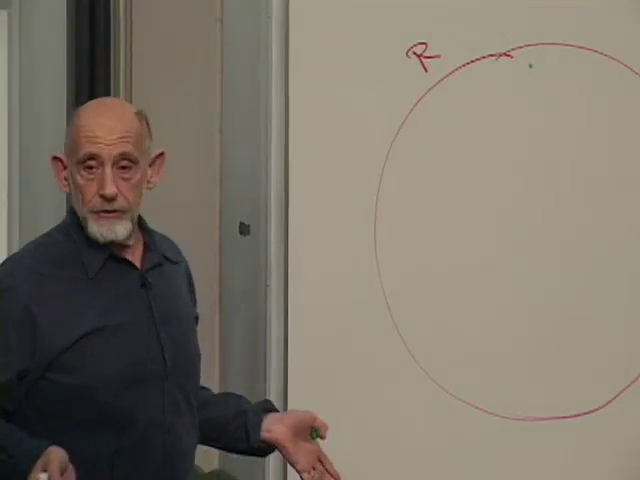
\includegraphics[width=0.74\textwidth]{lecture_09_figure_02.png}
  \caption{Die Kontrollrechnung für das Punktteilchen:
  \(p^2/(2m)=L^2/(2mR^2)=L^2/(2I)\).}
  \lectureframe{00:11:25}
  \label{fig:l09-sphere-rotor}
\end{figure}

Dieses unproblematische Beispiel ist wichtig. Die Krümmung an sich ist nicht das Problem. Es entsteht, wenn die Krümmung mit der inneren Quantenausdehnung einer Saite gekoppelt wird.

\section{Die Vakuumsaite ist kein Punkt}

Betrachten wir eine transversale Koordinate einer offenen Saite und ziehen ihren Schwerpunkt ab. Die hier verwendete Oszillatorentwicklung ist schematisch:
\begin{equation}
  X(\sigma)-X_{\mathrm{cm}}
  \sim
  \sum_{n=1}^{\infty}
  \frac{a_n+a_n^\dagger}{\sqrt n}\cos(n\sigma).
  \label{eq:l09-mode-expansion}
\end{equation}
Entscheidend sind die Kosinusmoden, die Oszillatoroperatoren und der Faktor \(1/\sqrt n\). Für die Abschätzung der Ausdehnung spielen die exakten Normierungen keine Rolle.
\editorialnote{Die genaue Entwicklung enthält von der Konvention abhängige Faktoren von \(\alpha'\), numerische Konstanten und eine bestimmte Notation für die Oszillatoren. Gleichung \eqref{eq:l09-mode-expansion} behält, wie bei der Herleitung an der Tafel, nur die für die UV-Abschätzung benötigte Abhängigkeit bei.}

\begin{figure}[H]
  \centering
  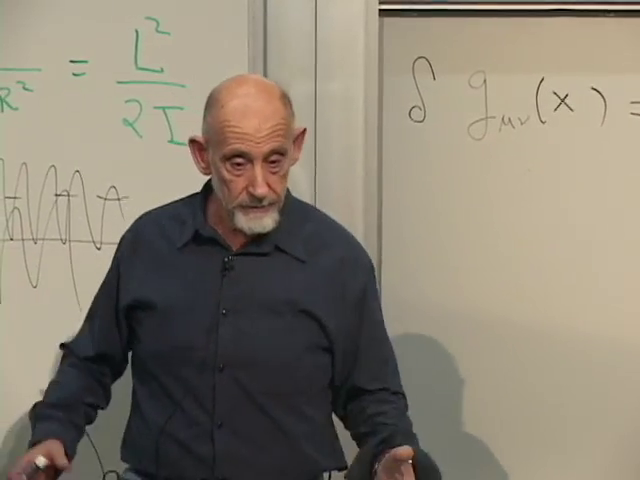
\includegraphics[width=0.78\textwidth]{lecture_09_figure_03.png}
  \caption{Die schematische Oszillatorentwicklung und die beim Quadrieren entstehende Doppelsumme.}
  \lectureframe{00:15:20}
  \label{fig:l09-string-modes}
\end{figure}

Der quadratische Abstand vom Schwerpunkt im Oszillatorvakuum ist
\begin{align}
  \expect{\bigl(X(\sigma)-X_{\mathrm{cm}}\bigr)^2}_0
  &\sim
  \sum_{n,m\geq1}
  \frac{\cos(n\sigma)\cos(m\sigma)}{\sqrt{nm}}\notag\\
  &\qquad\times
  \bra{0}(a_n+a_n^\dagger)\notag\\
  &\hspace{6em}\times(a_m+a_m^\dagger)\ket{0}.
  \label{eq:l09-size-double-sum}
\end{align}
Die meisten Terme verschwinden. Zwei Vernichtungsoperatoren wirken auf den Ket annihilierend; zwei Erzeugungsoperatoren erzeugen einen Zustand, der zum Bra orthogonal ist. Auch ein Erzeugungsoperator gefolgt von einem Vernichtungsoperator hat in dieser Reihenfolge einen verschwindenden Vakuumerwartungswert. Die verbleibende Kontraktion lautet
\begin{equation}
  \bra{0}a_n a_m^\dagger\ket{0}=\delta_{nm}.
  \label{eq:l09-vacuum-contraction}
\end{equation}

\begin{figure}[H]
  \centering
  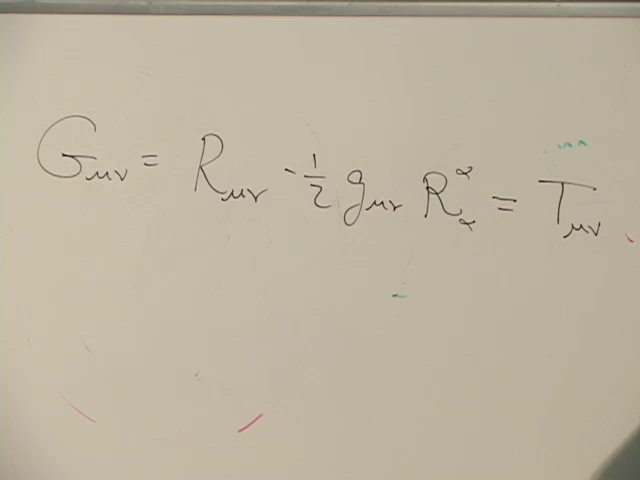
\includegraphics[width=0.74\textwidth]{lecture_09_figure_04.png}
  \caption{Die verbleibende Vakuumkontraktion reduziert die doppelte Oszillatorsumme auf eine einfache Summe.}
  \lectureframe{00:20:10}
  \label{fig:l09-vacuum-contraction}
\end{figure}

Damit gilt
\begin{equation}
  \expect{\bigl(X(\sigma)-X_{\mathrm{cm}}\bigr)^2}_0
  \sim
  \sum_{n=1}^{\infty}\frac{\cos^2(n\sigma)}{n}.
  \label{eq:l09-size-single-sum}
\end{equation}
An einem beliebigen Punkt der Saite oder nach einer Mittelung über \(\sigma\) trägt \(\cos^2(n\sigma)\) ungefähr \(1/2\) bei. Mit einer Modenabschneidung bei \(N\) gilt
\begin{equation}
  \expect{\bigl(X-X_{\mathrm{cm}}\bigr)^2}_{0,N}
  \sim
  \frac{1}{2}\sum_{n=1}^{N}\frac{1}{n}
  =\frac{1}{2}\log N+O(1).
  \label{eq:l09-logarithmic-size}
\end{equation}

\begin{figure}[H]
  \centering
  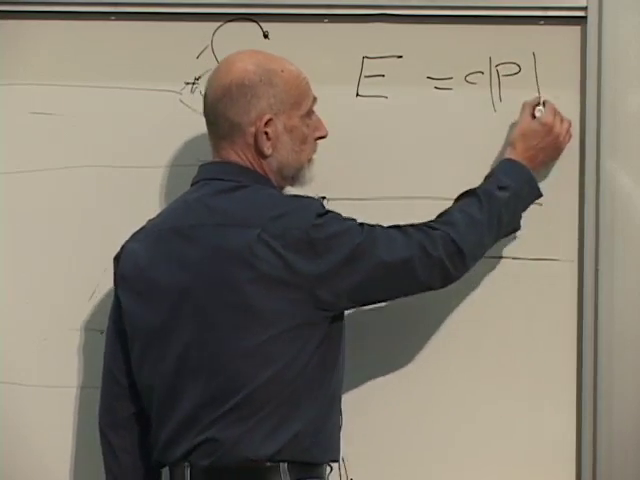
\includegraphics[width=0.72\textwidth]{lecture_09_figure_05.png}
  \caption{Die Herleitung an der Tafel führt auf die harmonische Summe, die die Ausdehnung des Grundzustands bestimmt.}
  \lectureframe{00:22:05}
  \label{fig:l09-harmonic-size}
\end{figure}

Beschränkt man sich etwa auf die ersten fünfundzwanzig Moden, erhält man ein verschwommenes Objekt endlicher Ausdehnung, aber noch nicht die Saite im Kontinuum. Wird die Abschneidung aufgehoben, wächst die mittlere quadratische Ausdehnung logarithmisch. Daraus darf man nicht schließen, die Stringtheorie im flachen Raum sei inkonsistent. Im flachen Raum entkoppeln die Schwerpunkt- und die Oszillatorbewegung, und heikle Auslöschungen in physikalischen Amplituden bewahren die erwartete Lokalität. Die wachsende Ausdehnung ist ein Warnsignal. Ob daraus ein Problem wird, zeigt die Krümmung.

\section{Wenn die innere Ausdehnung die Geometrie verändert}

Wir platzieren die Saite nahe dem Nordpol der Kugel. Sind alle Oszillatoren ausgeschaltet, verhält sie sich wie das soeben betrachtete Punktteilchen. Werden höhere Moden zugelassen, wird die Saite zu einem fluktuierenden Knäuel, das über die Kappe verteilt ist. Ihr Schwerpunkt kann sich weiterhin um die Kugel bewegen, doch das Objekt, dessen Trägheitsmoment in die Rotationsenergie eingeht, ist nun ausgedehnt.

Für eine Achse durch den Kugelmittelpunkt und die Pole gilt
\begin{equation}
  I=\int r_\perp^2\,dm,
  \label{eq:l09-extended-inertia}
\end{equation}
wobei \(r_\perp\) der senkrechte Abstand eines Saitenelements von dieser Achse ist. Ein Punkt am Äquator der Bahn hat den größten relevanten Hebelarm. Saitenabschnitte, die zur Achse hin absinken, tragen weniger bei. Bei fester Gesamtmasse verringert sich dadurch das effektive Trägheitsmoment:
\begin{equation}
  I_{\mathrm{eff}}<mR^2.
  \label{eq:l09-inertia-reduction}
\end{equation}
Die Rotationsenergie sieht daher so aus wie die eines Punktobjekts auf einer kleineren Kugel:
\begin{equation}
  E_{\mathrm{rot}}
  =\frac{L^2}{2I_{\mathrm{eff}}}
  \equiv \frac{L^2}{2mR_{\mathrm{eff}}^2},
  \qquad R_{\mathrm{eff}}<R.
  \label{eq:l09-effective-radius}
\end{equation}

\begin{classroomqa}
\audiencequestion{Warum sollte das Trägheitsmoment gegen null gehen, wenn sich die Saite über einen größeren Bereich ausdehnt? \lecturetimestamp{00:33:23}}
\lecturerresponse{Die Aussage bezieht sich auf die effektive Beschreibung nach wiederholtem Grobkörnen. Sie besagt nicht, dass die rohe ausgedehnte Verteilung unmittelbar ein verschwindendes Trägheitsmoment hat. Das erste Modenband macht aus dem Punkt eine verschwommene Ansammlung, die sich so bewegt, als läge sie auf einer kleineren Kugel. Das nächste Band löst die Struktur innerhalb jeder solchen Ansammlung auf und wiederholt dieselbe Renormierung. Durch die wiederholte Anwendung wandert der effektive Radius nach innen.}
\end{classroomqa}

\begin{figure}[H]
  \centering
  \includegraphics[width=0.72\textwidth]{lecture_09_figure_06.png}
  \medskip

  \begin{adjustbox}{max width=\linewidth}
  \begin{tikzpicture}[x=1cm,y=1cm,>=Latex]
    \draw[thick] (0,0) circle (2.15);
    \draw[dashed] (0,-2.55) -- (0,2.55);
    \draw[blue!65!black,thick]
      (-0.22,2.05)
      .. controls (-1.22,1.75) and (-1.52,1.08) .. (-1.06,0.44)
      .. controls (-0.55,-0.10) and (0.35,0.02) .. (1.10,0.68)
      .. controls (1.48,1.12) and (1.16,1.80) .. (0.20,2.05);
    \draw[red!70!black,dashed] (0,0) circle (1.25);
    \draw[->] (2.70,1.55) -- (4.05,1.55);
    \node[align=center] at (3.37,1.98) {add shorter\\modes};
    \draw[thick] (6.15,0) circle (1.25);
    \draw[dashed] (6.15,-1.65) -- (6.15,1.65);
    \draw[blue!65!black,thick]
      (6.00,1.18)
      .. controls (5.42,0.88) and (5.46,0.25) .. (6.02,-0.06)
      .. controls (6.46,-0.28) and (6.90,0.45) .. (6.28,1.18);
    \node at (0,-3.00) {sphere of radius \(R\)};
    \node at (6.15,-2.05) {effective radius \(R_{\mathrm{eff}}\)};
  \end{tikzpicture}
  \end{adjustbox}
  \caption{Die Saite am Nordpol aus der Tafelzeichnung und eine saubere Rekonstruktion des Arguments für den effektiven Radius. Der gestrichelte innere Kreis bezeichnet eine effektive Geometrie, keine zweite physische Schale innerhalb der Kugel.}
  \lectureframe{00:35:15}
  \label{fig:l09-shrinking-sphere}
\end{figure}

Dies ist eine Aussage über die Renormierungsgruppe. Bei endlicher Abschneidung ist die Saite ein Knäuel mit begrenzter innerer Auflösung. Eine Erhöhung der Abschneidung verändert die Mechanik dieses Knäuels. Auf einer positiv gekrümmten Kugel wird der aus der langreichweitigen Bewegung erschlossene Hintergrund mit jeder zusätzlich berücksichtigten Modenschale kleiner. Stabilisiert sich das Ergebnis nie, gibt es auf diesem Hintergrund keine abschneidungsunabhängige Stringtheorie.

\section{Die Metrik muss einen Fixpunkt erreichen}

Ersetzen wir nun die Kugel durch eine allgemeine Zielraummetrik \(g_{\mu\nu}(x)\). Die Integration über eine dünne logarithmische Schale von Oszillatormoden verändert diese Metrik um einen lokalen symmetrischen Tensor vom Rang zwei. Die Änderung muss im flachen Raum verschwinden und mit zwei Ableitungen der Metrik beginnen. In führender Ordnung lässt die Kovarianz als maßgeblichen Kandidaten den Ricci-Tensor übrig:
\begin{equation}
  \frac{\partial g_{\mu\nu}}{\partial\log\Lambda}
  =-C\,R_{\mu\nu}+\cdots ,
  \qquad C>0
  \label{eq:l09-ricci-flow}
\end{equation}
in der Richtung der Grobkörnung, die im geometrischen Argument verwendet wird. Positive Krümmung lässt eine Kugel dadurch wie erforderlich schrumpfen.
\editorialnote{Normierung und Vorzeichen hängen davon ab, ob der Renormierungsparameter in Richtung UV oder IR zunimmt. In der üblichen Weltenblattnotation lautet die führende Metrik-Betafunktion \(\beta^g_{\mu\nu}=\alpha'R_{\mu\nu}+\cdots\). Die hier verwendete invariante Aussage lautet: Abschneidungsunabhängigkeit erfordert, dass die Betafunktion und damit in dieser Ordnung \(R_{\mu\nu}\) verschwindet.}

\begin{figure}[H]
  \centering
  \includegraphics[width=0.76\textwidth]{lecture_09_figure_07.png}
  \caption{Die Metrikänderung ist schematisch als minus Ricci-Tensor dargestellt, daneben eine eingezeichnete Glättungskurve.}
  \lectureframe{00:43:00}
  \label{fig:l09-ricci-flow-board}
\end{figure}

\begin{classroomqa}
\audiencequestion{Wo tritt die Oszillatorabschneidung \(N\) in dieser Flussgleichung auf? \lecturetimestamp{00:43:38}}
\lecturerresponse{Sie ist die Skalenvariable. Die Summe für die Saitenausdehnung ändert sich logarithmisch mit der höchsten einbezogenen Mode. Daher ist der natürliche Entwicklungsparameter \(\log N\) oder äquivalent \(\log\Lambda\). Gleichung \eqref{eq:l09-ricci-flow} beschreibt die infinitesimale Änderung, die eine logarithmische Modenschale hervorruft.}
\end{classroomqa}

Ein zulässiger Hintergrund ist ein Fixpunkt dieses Flusses. In führender Ordnung gilt
\begin{equation}
  \boxed{R_{\mu\nu}=0.}
  \label{eq:l09-ricci-flat}
\end{equation}
Ricci-flach bedeutet nicht, dass jede Komponente des Riemann-Tensors verschwindet. Gravitationswellen können beispielsweise im Vakuum eine von null verschiedene Krümmung haben und zugleich \(R_{\mu\nu}=0\) erfüllen.

\subsection{Dieselbe Bedingung ist die Vakuum-Einstein-Gleichung}

Unter Weglassung der üblichen Konstanten lautet Einsteins Gleichung
\begin{equation}
  G_{\mu\nu}
  \equiv
  R_{\mu\nu}-\frac12 g_{\mu\nu}R
  =T_{\mu\nu}.
  \label{eq:l09-einstein}
\end{equation}

\begin{figure}[H]
  \centering
  \includegraphics[width=0.78\textwidth]{lecture_09_figure_08.png}
  \caption{Einstein-Tensor und Energie-Impuls-Tensor an der Tafel.}
  \lectureframe{00:47:15}
  \label{fig:l09-einstein-board}
\end{figure}

Im Vakuum gilt \(T_{\mu\nu}=0\). Die Spur von \(D\) Raumzeitdimensionen ergibt
\begin{equation}
  0=g^{\mu\nu}G_{\mu\nu}
   =\left(1-\frac{D}{2}\right)R.
  \label{eq:l09-einstein-trace}
\end{equation}
Für \(D\neq2\) gilt also \(R=0\); setzt man dies in \eqref{eq:l09-einstein} ein, erhält man \(R_{\mu\nu}=0\). Die Bedingung, dass die Saite ihre Abhängigkeit von der Abschneidung verliert, ist somit die Vakuum-Feldgleichung der Gravitation. Die Gravitation wurde der Theorie nicht nachträglich hinzugefügt; sie ergibt sich als Preis der Konsistenz.

Das Wort \emph{Vakuum} bedeutet nicht, dass nichts geschieht. Es bedeutet, dass es im betrachteten Gebiet keine Quelle des Energie-Impuls-Tensors gibt. Die quellfreien Maxwell-Gleichungen lassen elektromagnetische Wellen zu, und die quellfreien Einstein-Gleichungen lassen Gravitationswellen zu. Die Geometrie kann dynamisch sein, obwohl ihr Ricci-Tensor verschwindet.

\begin{classroomqa}
\audiencequestion{Hängt diese Bedingung mit der konformen Invarianz zusammen?\lecturetimestamp{00:52:20}}
\lecturerresponse{Ja, obwohl die Frage in der Aufzeichnung teilweise unverständlich ist. Die relevante Symmetrie ist die konforme Invarianz der quantenmechanischen \emph{Weltenblatt}-Theorie. Die Forderung, dass die Skalenanomalie des Weltenblatts verschwindet, setzt die Metrik-Betafunktion auf null. Das ist nicht mit der Forderung zu verwechseln, dass die Raumzeit selbst konform invariant ist.}
\end{classroomqa}

Es gibt eine zweite Konsistenzbedingung. Die konforme Invarianz des Weltenblatts legt auch die kritische Raumzeitdimension fest: zehn für Superstrings und sechsundzwanzig für die bosonische Saite. Ricci-Flachheit ist daher nicht die vollständige Liste der Anforderungen, aber sie ist der Teil, an dem die Einstein-Gleichung am unmittelbarsten sichtbar wird.

\section{Kompakte Dimensionen statt fehlender Dimensionen}

Ein Superstring-Hintergrund besitzt neun Raumdimensionen und eine Zeitdimension. In unserer makroskopischen Welt sind nur drei große Raumrichtungen sichtbar. Sechs Raumdimensionen müssen daher verborgen oder auf andere Weise auf gewöhnlichen Skalen unzugänglich sein. Durch Kompaktifizierung bleiben sie echte Richtungen, erhalten aber eine kleine, endliche Ausdehnung.

\begin{classroomqa}
\audiencequestion{Bedeutet es, mehr als eine Zeitdimension zu haben, wenn verschiedene Beobachter unterschiedliche Uhren mitführen? \lecturetimestamp{00:56:59}}
\lecturerresponse{Nein. Viele Uhren sind viele Instrumente, die Koordinaten in einer Raumzeit messen; sie erzeugen keine voneinander unabhängigen zeitartigen Richtungen. Die hier betrachteten zusätzlichen Dimensionen sind räumlich. Die bekannten quantenmechanischen und kausalen Konstruktionen liefern keine vergleichbar konsistente Theorie mit mehreren lokalen Zeitrichtungen. Diese Möglichkeit gehört daher nicht zu diesem Kompaktifizierungsmodell.}
\end{classroomqa}

Stellen wir uns Wesen vor, die glauben, ihre Welt sei eine Linie. Bei niedriger Auflösung können sie sich nur vorwärts und rückwärts bewegen. Unter einem hinreichend leistungsfähigen Mikroskop zeigt sich jedoch, dass die Linie ein sehr dünner Zylinder ist. Ein kleines Wesen kann sich sowohl entlang seiner Länge als auch um seine Kreisrichtung bewegen. Die zweite Richtung war schon immer vorhanden; ihr Umfang war für grobe Sonden zu klein, um aufgelöst zu werden.

\begin{figure}[H]
  \centering
  \includegraphics[width=0.78\textwidth]{lecture_09_figure_09.png}
  \caption{Ein schmaler Zylinder und Bahnen, die sich um seine verborgene Kreisrichtung winden.}
  \lectureframe{01:01:00}
  \label{fig:l09-hidden-cylinder}
\end{figure}

Ein Zylinder lässt sich als Streifen darstellen, dessen obere und untere Kante identifiziert werden. Beim Überschreiten der oberen Kante gelangt man an derselben Position entlang des Zylinders durch die untere Kante zurück. An keiner der beiden Kanten gibt es einen physikalischen Rand. Dasselbe lässt sich in zwei Richtungen durchführen: Man identifiziert sowohl die linke mit der rechten als auch die obere mit der unteren Kante eines Rechtecks. Das Ergebnis ist ein Zweitorus.

\begin{figure}[H]
  \centering
  \includegraphics[width=0.76\textwidth]{lecture_09_figure_10.png}
  \medskip

  \begin{tikzpicture}[x=0.82cm,y=0.82cm,>=Latex]
    \draw[thick] (0,0) rectangle (4,2.15);
    \draw[blue!65!black,->] (0,2.48) -- (4,2.48);
    \draw[blue!65!black,->] (4,-0.34) -- (0,-0.34);
    \node at (2,-0.82) {one periodic direction};
    \draw[thick] (6.1,0) rectangle (10.1,2.15);
    \draw[blue!65!black,->] (6.1,2.48) -- (10.1,2.48);
    \draw[blue!65!black,->] (10.1,-0.34) -- (6.1,-0.34);
    \draw[red!70!black,->] (5.76,0) -- (5.76,2.15);
    \draw[red!70!black,->] (10.44,2.15) -- (10.44,0);
    \node at (8.1,-0.82) {two periodic directions};
  \end{tikzpicture}
  \caption{Die Quaderdarstellung an der Tafel und eine klare Beschreibung des Fundamentalbereichs. Identifiziert man ein Kantenpaar, entsteht ein Zylinder; identifiziert man beide Paare, entsteht ein Torus.}
  \lectureframe{01:04:40}
  \label{fig:l09-periodic-identification}
\end{figure}

Der Torus ist zunächst ein topologischer Raum und erst danach eine donutförmige Fläche im dreidimensionalen Raum. Schneidet man einen Torus einmal auf, erhält man einen Zylinder; ein weiterer Schnitt ergibt ein Rechteck, sofern man die Kantenidentifikationen im Gedächtnis behält. Auf dieses Rechteck lässt sich eine flache Metrik legen. Der so entstehende flache Torus hat lokal verschwindende Riemann-Krümmung und ist daher sicher Ricci-flach.

Eine gerade Bahn auf dem Rechteck setzt sich über eine identifizierte Kante hinweg gerade fort. Ist ihre Steigung ein rationales Verhältnis der beiden Perioden, schließt sich die Bahn schließlich. Ist das Verhältnis irrational, schließt sie sich nie und liegt dicht auf dem Torus.

\begin{figure}[H]
  \centering
  \includegraphics[width=0.76\textwidth]{lecture_09_figure_11.png}
  \caption{Wiederholte gerade Abschnitte im Fundamentalbereich stellen eine einzige, ununterbrochene Bahn auf dem Torus dar.}
  \lectureframe{01:11:00}
  \label{fig:l09-torus-trajectory}
\end{figure}

Tori höherer Dimension entstehen auf dieselbe Weise. Ein Würfel, bei dem jeweils gegenüberliegende Seitenflächen identifiziert werden, ist ein Dreitorus; sechs kompakte Richtungen lassen sich durch einen Sechstorus modellieren. Man sollte nicht versuchen, all diese Objekte in den gewöhnlichen dreidimensionalen Raum einzubetten. Die Beschreibung durch die Identifikation der Seitenflächen ist intrinsisch und vollständig.

\begin{classroomqa}
\audiencequestion{Muss sich eine zusätzliche Dimension notwendigerweise in sich selbst zurückschließen?\lecturetimestamp{01:15:03}}
\lecturerresponse{Das ist kein Satz. Sie könnte nichtkompakt sein, würde sich dann aber normalerweise als weitere große Richtung in der beobachteten Welt auf großen Distanzen bemerkbar machen. Kompaktheit ist die einfachste Möglichkeit, zusätzliche Dimensionen mit ihrem scheinbaren Fehlen in Einklang zu bringen. Warum die Natur eine bestimmte Kompaktifizierung wählt, ist eine eigene dynamische Frage.}
\end{classroomqa}

\begin{classroomqa}
\audiencequestion{Warum nehmen wir an, dass die unbeobachteten Dimensionen gewöhnliche Raumrichtungen sind, die auf diese Weise aufgerollt sind, und nicht etwas ganz anderes? \lecturetimestamp{01:15:51}}
\lecturerresponse{Weil dies eine konkrete, lösbare Hypothese ist, nicht weil bewiesen wäre, dass sie die einzig mögliche Beschreibung der Natur ist. Kompakte räumliche Mannigfaltigkeiten ermöglichen es uns, konsistente Beispiele zu konstruieren und ihre Spektren zu berechnen. Exotischere Möglichkeiten müssen sich durch dasselbe auszeichnen.}
\end{classroomqa}

\begin{classroomqa}
\audiencequestion{Die Abstände auf dem vertrauten, donutförmigen Torus sehen nicht wie Abstände in einem Rechteck aus. Welche Geometrie ist gemeint?
\lecturetimestamp{01:18:11}}
\lecturerresponse{Der Begriff \emph{Torus} legt die Identifikationen fest, aber keine eindeutige Metrik. Der eingebettete Donut erbt eine gekrümmte Metrik aus dem dreidimensionalen Raum. Das periodisch identifizierte Rechteck trägt eine flache Metrik. Beide haben dieselbe Topologie, aber verschiedene Geometrien. Bei der einfachen Kompaktifizierung meinen wir die flache Geometrie.}
\end{classroomqa}

\section{Die Formparameter eines flachen Torus}

Selbst ein flacher Zweitorus ist nicht eindeutig. Sein Fundamentalparallelogramm hat eine Gesamtfläche, ein Seitenverhältnis und eine Scherung. Änderungen dieser Parameter verändern die Abstände und damit das Spektrum, ohne die Topologie zu ändern.

\begin{figure}[H]
  \centering
  \includegraphics[width=0.74\textwidth]{lecture_09_figure_12.png}
  \medskip

  \begin{tikzpicture}[x=0.9cm,y=0.9cm,>=Latex]
    \draw[thick] (0,0) rectangle (3.4,2.1);
    \draw[<->] (0,-0.35) -- node[below] {\(L_1\)} (3.4,-0.35);
    \draw[<->] (-0.35,0) -- node[left] {\(L_2\)} (-0.35,2.1);
    \draw[thick] (5.4,0) -- (8.8,0) -- (9.7,2.1) -- (6.3,2.1) -- cycle;
    \draw[dashed] (5.4,0) -- (6.3,2.1);
    \draw[->] (5.75,2.48) -- node[above] {shear} (6.45,2.48);
    \node at (1.7,-1.00) {area and aspect ratio};
    \node at (7.55,-1.00) {complex structure};
  \end{tikzpicture}
  \caption{Die rechteckigen und gescherten Fundamentalbereiche zur Beschreibung der Torusmoduli.}
  \lectureframe{01:23:00}
  \label{fig:l09-torus-moduli}
\end{figure}

Für einen Zweitorus lässt sich die Form zweckmäßig durch eine komplexe Zahl \(\tau=\tau_1+i\tau_2\) beschreiben: Der Realteil gibt die Scherung an, der Imaginärteil nach Abspaltung eines Gesamtmaßstabs das Seitenverhältnis. Durch Vertauschen der beiden grundlegenden Zyklen oder eine Änderung ihrer ganzzahligen Basis können scheinbar verschiedene Parallelogramme denselben Torus beschreiben.

\begin{classroomqa}
\audiencequestion{Was passiert, wenn eine Kante vor der Identifikation umgeklappt wird? \lecturetimestamp{01:24:20}}
\lecturerresponse{Das ergibt eine andere Topologie. Eine Identifikation mit Spiegelung erzeugt eine nichtorientierbare Fläche, die Kleinsche Flasche, statt eines gewöhnlichen Torus.}
\end{classroomqa}

\begin{classroomqa}
\audiencequestion{Was geschieht, wenn die Verdrehung entlang der Kante nicht gleichmäßig ist?
\lecturetimestamp{01:25:01}}
\lecturerresponse{Eine glatte, nicht gleichmäßige Verformung lässt sich in die Metrik des Fundamentalbereichs übertragen. Die topologische Identifikation und die geometrischen Daten müssen auseinandergehalten werden: Eine Änderung der Verklebung kann die Topologie ändern, während eine glatte Änderung der Abstände die Metrik verändert.}
\end{classroomqa}

\editorialnote{Bei einem flachen Zweitorus ist die Fläche der einfachste Kähler-Modul, und \(\tau\) ist das Modul der komplexen Struktur. Eine kontinuierliche Scherung gehört zu \(\tau\). Ein Dehn-Twist ist dagegen eine diskrete Operation der Abbildungsklassengruppe, dargestellt durch \(\tau\mapsto\tau+1\); er ist selbst kein kontinuierlicher Modul. Damit wird die bewusst informelle Terminologie aus der Diskussion an der Tafel präzisiert.}

Flache Tori sind nützlich, weil sie die Konsistenzbedingung unmittelbar erfüllen. Ihre Symmetrie ist jedoch zu groß, um ein realistisches Modell der Teilchenphysik zu liefern. Kompliziertere Ricci-flache Räume, insbesondere Calabi--Yau-Mannigfaltigkeiten, ermöglichen vielfältigere Kompaktifizierungen. Ihre detaillierte Konstruktion geht über diese Diskussion hinaus; das Prinzip bleibt dasselbe.

\section{Eine kompakte Kreisdimension aus ihrem Spektrum ablesen}

Nach der Pause reduzieren wir den kompakten Raum auf einen Kreis mit Umfang \(2\pi R\). Eine Wellenfunktion muss nach einem Umlauf eindeutig sein:
\begin{equation}
  e^{ip_c(x+2\pi R)/\hbar}=e^{ip_cx/\hbar}.
\end{equation}
Daraus folgt
\begin{equation}
  p_cR=n\hbar,
  \qquad
  p_c=\frac{n\hbar}{R},
  \qquad n\in\mathbb Z.
  \label{eq:l09-kk-momentum}
\end{equation}

\begin{figure}[H]
  \centering
  \includegraphics[width=0.74\textwidth]{lecture_09_figure_13.png}
  \caption{Der kompakte Umfang \(2\pi R\) und der quantisierte Impuls \(p_c=n\hbar/R\).}
  \lectureframe{01:32:15}
  \label{fig:l09-kk-board}
\end{figure}

Für ein masseloses Teilchen in der vollständigen Raumzeit gilt
\begin{equation}
  E=c|\mathbf P|.
  \label{eq:l09-massless-dispersion}
\end{equation}

\begin{figure}[H]
  \centering
  \includegraphics[width=0.70\textwidth]{lecture_09_figure_14.png}
  \caption{Die Dispersionsrelation für ein masseloses Teilchen, mit der der kompakte Impuls als Masse in niedrigerer Dimension umgedeutet wird.}
  \lectureframe{01:33:45}
  \label{fig:l09-massless-board}
\end{figure}

Wir zerlegen den Impuls in nichtkompakte und kompakte Anteile und setzen \(c=\hbar=1\):
\begin{equation}
  E^2=\mathbf p_{\mathrm{large}}^2+\frac{n^2}{R^2}.
  \label{eq:l09-kk-dispersion}
\end{equation}
Ein Beobachter, der die kompakte Richtung nicht auflösen kann, vergleicht dies mit \(E^2=\mathbf p_{\mathrm{large}}^2+m^2\) und erschließt daraus einen Massenturm:
\begin{equation}
  m_n=\frac{|n|}{R}.
  \label{eq:l09-kk-masses}
\end{equation}
Die beiden Vorzeichen von \(n\) beschreiben entgegengesetzte kompakte Impulse mit derselben positiven Energie, nicht positive und negative Massen. Der Abstand \(1/R\) gibt daher spektroskopisch den Radius zu erkennen. Das ist der Kaluza--Klein-Mechanismus: Der Impuls in einer verborgenen Richtung erscheint in den sichtbaren Dimensionen als Masse.

\section{Wicklungszustände vervollständigen das Spektrum}

Eine geschlossene Saite kann etwas, das einem Punktteilchen nicht möglich ist: Sie kann sich um den Kreis wickeln. Ist die Wicklungszahl \(w\), schließt sich die Saite erst, nachdem sie die kompakte Richtung \(w\)-mal durchlaufen hat. Ihre Länge beträgt \(2\pi |w|R\), sodass die Spannung eine Energie liefert:
\begin{equation}
  m_w
  =2\pi T\,|w|R
  =\frac{|w|R}{\alpha'}.
  \label{eq:l09-winding-mass}
\end{equation}
In der Vorlesung werden Einheiten mit \(\alpha'=1\) gewählt; damit vereinfacht sich dies zu
\begin{equation}
  m_w=|w|R.
  \label{eq:l09-winding-lecture-units}
\end{equation}
Positive und negative Werte von \(w\) entsprechen entgegengesetzten Umlaufrichtungen um den Kreis.

\begin{figure}[H]
  \centering
  \includegraphics[width=0.76\textwidth]{lecture_09_figure_15.png}
  \caption{Eine geschlossene Saite, die um den kompakten Zylinder gewickelt ist; der kompakte Radius ist an der Tafel markiert.}
  \lectureframe{01:39:45}
  \label{fig:l09-winding-board}
\end{figure}

Der kompakte Kreis erzeugt somit zwei einander ergänzende Spektren:
\begin{equation}
  m_n=\frac{|n|}{R},
  \qquad
  m_w=\frac{|w|R}{\alpha'}.
  \label{eq:l09-two-towers}
\end{equation}
Ist \(R\) groß, liegen die Impulsniveaus dicht beieinander und die Wicklungszustände sind schwer. Ist \(R\) klein, liegen die Impulsniveaus weit auseinander und die Wicklungszustände sind leicht.

\begin{figure}[H]
  \centering
  \begin{tikzpicture}[x=1cm,y=0.9cm,>=Latex]
    \draw[->] (0,0) -- (0,4.7) node[above] {\(m\)};
    \foreach \y/\lab in {0/0,1.1/{1/R},2.2/{2/R},3.3/{3/R},4.4/{4/R}} {
      \draw (-0.16,\y) -- (0.16,\y);
      \node[left] at (-0.22,\y) {\(\lab\)};
    }
    \node at (0,-0.62) {momentum};
    \draw[<->,very thick,blue!65!black] (2.05,2.15) -- (4.05,2.15)
      node[midway,above] {\(R\leftrightarrow\alpha'/R\)};
    \draw[->] (6.1,0) -- (6.1,4.7) node[above] {\(m\)};
    \foreach \y/\lab in {0/0,1.1/{R/\alpha'},2.2/{2R/\alpha'},3.3/{3R/\alpha'},4.4/{4R/\alpha'}} {
      \draw (5.94,\y) -- (6.26,\y);
      \node[right] at (6.32,\y) {\(\lab\)};
    }
    \node at (6.1,-0.62) {winding};
  \end{tikzpicture}
  \caption{Bei Inversion des Radius in Stringeinheiten werden die Impuls- und Wicklungstürme vertauscht.}
  \label{fig:l09-dual-mass-towers}
\end{figure}

\section{T-Dualität: Kleine und große Kreise beschreiben dieselbe Physik}

Die beiden Spektren werden durch folgende Zuordnung ineinander überführt:
\begin{equation}
  R\longleftrightarrow\frac{\alpha'}{R},
  \qquad
  n\longleftrightarrow w.
  \label{eq:l09-t-duality}
\end{equation}
In den an der Tafel verwendeten Einheiten gilt \(\alpha'=1\); daher ist dies einfach \(R\leftrightarrow1/R\). Beim selbstdualen Radius \(R=\sqrt{\alpha'}\) stimmen die Impuls- und Wicklungsskalen überein.

\begin{figure}[H]
  \centering
  \includegraphics[width=0.74\textwidth]{lecture_09_figure_16.png}
  \caption{Die an der Tafel verglichenen dünnen und dichten Massenspektren, wenn der Radius die selbstduale Skala überschreitet.}
  \lectureframe{01:43:00}
  \label{fig:l09-duality-board}
\end{figure}

Der Austausch der elementaren Massenformeln ist nur der sichtbare Teil des Ergebnisses. Auch geschlossene Saiten-Oszillatorzustände und Streuamplituden werden konsistent ineinander überführt. Ein Kreis, der kleiner als die Stringskala ist, beschreibt keine neue, immer winzigere Geometrie; er besitzt eine äquivalente Beschreibung durch einen größeren dualen Kreis. Punktteilchen können diese Identifikation nicht erfüllen, weil sie zwar Impulsmoden, aber keine Wicklungsmoden besitzen.

\begin{classroomqa}
\audiencequestion{Ist das nicht einfach dasselbe, wie eine vertikale und eine horizontale Richtung zu vertauschen? \lecturetimestamp{01:44:38}}
\lecturerresponse{Nein. Vertauscht werden zwei verschiedene Quantenzahlen: der Impuls um den Kreis und die Anzahl der Umläufe einer geschlossenen Saite um den Kreis. Gleichzeitig muss der Radius invertiert werden.}
\end{classroomqa}

\begin{classroomqa}
\audiencequestion{Beziehen sich die Beschreibungen bei \(R<\sqrt{\alpha'}\) und \(R>\sqrt{\alpha'}\) nur auf Bosonen oder auch auf Fermionen?
\lecturetimestamp{01:46:30}}
\lecturerresponse{Die Dualität ist eine Symmetrie der vollständigen kompaktifizierten Stringtheorie und nicht bloß des einfachen bosonischen Massenspektrums, an dem sie veranschaulicht wird. Die genaue Zuordnung der Sektoren hängt von der Theorie ab, doch die Äquivalenz zwischen kleinen -- und großen Radien ist nicht auf eine Teilchensorte beschränkt.}
\end{classroomqa}

\begin{classroomqa}
\audiencequestion{Vergleichen wir offene oder geschlossene Saiten? \lecturetimestamp{01:47:32}}
\lecturerresponse{Es sind Zustände geschlossener Saiten. Eine frei propagierende geschlossene Saite kann um einen kompakten Kreis gewickelt sein. Eine gewöhnliche offene Saite mit freien Enden trägt nicht dieselbe erhaltene Wicklungszahl.}
\end{classroomqa}
\editorialnote{In der umfassenderen Behandlung offener Saiten vertauscht die T-Dualität Neumann- und Dirichlet-Randbedingungen und führt D-Branen ein. Deshalb ist die T-Dualität offener Saiten umfassender, als einfach die Wicklungsformel für geschlossene Saiten zu übernehmen.}

\begin{classroomqa}
\audiencequestion{Ist dieser Austausch vergleichbar mit dem Austausch von Raum und Zeit nahe einem Schwarzen-Loch-Horizont? \lecturetimestamp{01:48:00}}
\lecturerresponse{Nein. Horizontkoordinaten und kausaler Charakter betreffen eine andere Frage. Hier beziehen sich die beiden Beschreibungen auf einen einzigen kompakten Raumkreis und den Austausch seiner Impuls- und Wicklungssektoren.}
\end{classroomqa}

\begin{classroomqa}
\audiencequestion{Löst dies das Problem der kurzreichweitigen Selbstenergie, indem es eine Mindestlänge liefert? \lecturetimestamp{01:48:35}}
\lecturerresponse{Es zeigt, dass Radien unterhalb der Stringskala keine neuen, nicht äquivalenten Kreis-Hintergründe beschreiben: Wenn \(R\) über den selbstdualen Punkt hinaus abnimmt, wächst der duale Radius. Das ist ein präzises stringtheoretisches Hindernis für die Untersuchung beliebig kleiner Kreisgeometrien. Daraus sollte man jedoch nicht folgern, jede denkbare Abstandsdefinition habe eine universelle, scharfe Untergrenze.}
\end{classroomqa}

\section{Warum Wicklungssektoren nicht weggelassen werden können}

\begin{classroomqa}
\audiencequestion{Könnten wir die Theorie ausschließlich mit windungsfreien Strings formulieren und die Windungszustände außen vor lassen? \lecturetimestamp{01:48:56}}
\lecturerresponse{Nein. Wechselwirkungen geschlossener Strings erzeugen sie. Dehnt man eine windungsfreie Schleife um die kompakte Richtung, sodass ein Abschnitt den Kreis in die eine und ein anderer Abschnitt ihn in die entgegengesetzte Richtung durchläuft, ist die Gesamtwindung weiterhin null. Bei einer Wiederverbindung kann sich die Schleife dann in zwei geschlossene Strings mit den Windungen \(+1\) und \(-1\) aufspalten. Das Paar kann sich voneinander entfernen. Daher müssen Windungszustände zum Spektrum gehören, selbst wenn der Anfangszustand keine enthielt.}
\end{classroomqa}

\begin{figure}[H]
  \centering
  \includegraphics[width=0.74\textwidth]{lecture_09_figure_17.png}
  \caption{Die gedehnte, windungsfreie Schleife, vor der Wiederverbindung um die kompakte Richtung gelegt.}
  \lectureframe{01:50:30}
  \label{fig:l09-winding-pair-before}
\end{figure}

\begin{figure}[H]
  \centering
  \includegraphics[width=0.72\textwidth]{lecture_09_figure_18.png}
  \medskip

  \begin{tikzpicture}[x=0.9cm,y=0.9cm,>=Latex]
    \draw[thick] (0,0) ellipse (1.0 and 1.55);
    \draw[blue!65!black,thick]
      (0.08,1.35) .. controls (2.0,1.15) and (2.0,-1.15) .. (0.08,-1.35);
    \draw[red!70!black,thick]
      (-0.08,-1.35) .. controls (-2.0,-1.15) and (-2.0,1.15) .. (-0.08,1.35);
    \node at (0,-2.15) {net \(w=0\)};
    \draw[->,thick] (2.45,0) -- (3.75,0) node[midway,above] {split};
    \draw[thick] (5.05,0.62) ellipse (0.68 and 1.02);
    \draw[blue!65!black,very thick,->]
      (5.05,1.64) arc[start angle=90,end angle=-250,x radius=0.68,y radius=1.02];
    \node at (5.05,-0.82) {\(w=+1\)};
    \draw[thick] (7.45,0.62) ellipse (0.68 and 1.02);
    \draw[red!70!black,very thick,<-]
      (7.45,1.64) arc[start angle=90,end angle=-250,x radius=0.68,y radius=1.02];
    \node at (7.45,-0.82) {\(w=-1\)};
  \end{tikzpicture}
  \caption{Die getrennte gewundene Schleife auf der Tafel und eine saubere Rekonstruktion der Erzeugung eines Windungs--Antiwindungs-Paares. Die Gesamtwindung bleibt null.}
  \lectureframe{01:51:30}
  \label{fig:l09-winding-pair-after}
\end{figure}

\begin{classroomqa}
\audiencequestion{Erfordert die Erzeugung des Windungspaares zusätzliche Energie?
\lecturetimestamp{01:52:11}}
\lecturerresponse{Ja. Das Dehnen eines Strings kostet Spannungsenergie, und die gewundenen Strings im Endzustand haben die in \eqref{eq:l09-winding-mass} angegebenen Massen. Eine hinreichend energiereiche Kollision kann das Paar erzeugen, ebenso wie eine Kollision ein Teilchen und sein Antiteilchen erzeugen kann, wobei die betreffende Erhaltungsgröße erhalten bleibt.}
\end{classroomqa}

\section{Kann man die Form eines String-Hintergrunds hören?}

Bei einer gewöhnlichen kompaktifizierten Teilchentheorie lässt sich aus dem Abstand des Kaluza--Klein-Spektrums der Radius erschließen: Man versucht, die Form des kompakten Raums aus seinen Normalmoden herauszuhören. In der Stringtheorie ist das Umkehrproblem subtiler. Impulsmoden geben Aufschluss über \(1/R\), Windungsmoden über \(R/\alpha'\), und das vollständige Spektrum bleibt unverändert, wenn man beide vertauscht. Zwei Radien, die in der Punktteilchengeometrie als verschieden gelten, beschreiben denselben String-Hintergrund in dualen Variablen.

Damit ist die Vorlesung auf einem Weg zu beiden angekündigten Schlussfolgerungen gelangt. Die Konsistenz im Ultraviolett zwingt die Zielraum-Metrik, der Vakuum-Einstein-Gleichung zu genügen; Gravitation ist daher unvermeidlich. Durch die Kompaktifizierung wird verborgene Geometrie in Teilchenspektren übersetzt, doch Windungszustände verhindern, dass dieses Spektrum unterhalb der Stringskala einen eindeutigen klassischen Radius festlegt. Die Konsistenz entscheidet nicht nur, welche Geometrien zulässig sind; durch T-Dualität verändert sie auch, was überhaupt als eigenständige Geometrie gilt.